% questions.tex —— 1988 年·广东卷·文史类 · 题目内容片段（无答案）
% 由 tools/generate_projects.py 依来源总账自 1988/1988_数学真题_广东文_试题.md 生成，勿手改（改源 MD 后重跑）


\gkpart{试题}

\begin{gktip}
\textbf{来源说明}：本题面依据固定源 PDF《一九八八年全国普通高等学校招生统一考试广东省数学试题与解答（文史类）》逐题转录。固定源共 21 页，PDF 第 1—7 页为题面，第 8—21 页为答案与解答。

\textbf{记号说明}：固定源使用 $\operatorname{tg}$、$\operatorname{ctg}$、$\operatorname{sec}$ 等记号，本文保留其含义并用 LaTeX 规范排版。第 24 小题的图形依据固定源重绘为 TikZ；第 3 题的几何图也依据固定源重绘为 TikZ。
\end{gktip}

\Needspace{0.4\textheight}
\begin{question}
\gkti{1}

第一卷满分 50 分，共有 25 个选择题。每题都给出代号为 A、B、C、D 的四个结论，其中只有一个结论正确。每题选对得 2 分，不选、选错或者选出的代号超过一个，一律得 0 分。

（1） 在等比数列 $\{a_n\}$ 中，已知 $a_7=6$，$a_9=9$，那么 $a_5=$\mbox{（　　）}

（A）$3$　　（B）$4$　　（C）$\dfrac32$　　（D）$2$

\Needspace{5\baselineskip}
（2） 指数方程

\nopagebreak[4]
\[
2+3^{x-1}=9^{x-\frac12}
\]

的解是\mbox{（　　）}

（A）$0$　　（B）$1$　　（C）$2$　　（D）$\dfrac12$

（3） 直线 $3x-2y=6$ 在 $y$ 轴上的截距是\mbox{（　　）}

（A）$3$　　（B）$-3$　　（C）$2$　　（D）$\dfrac32$

\Needspace{5\baselineskip}
（4） 设

\nopagebreak[4]
\[
P=\left\{x\mathrel{}\middle|\mathrel{}x=\sin\frac{m\pi}{6},\ m\in\mathbb N\right\},\qquad
Q=\left\{x\mathrel{}\middle|\mathrel{}x=\sin\frac{n\pi}{12},\ n\in\mathbb N\right\}.
\]

那么，关于集合 $P$ 和 $Q$ 有\mbox{（　　）}

（A）$P\supset Q$　　（B）$P\subset Q$

（C）$P=Q$　　（D）$P\cap Q=\varnothing$

（5） 用 $1\text{、}2\text{、}3\text{、}4\text{、}5$ 这五个数字，组成没有重复数字的五位数，那么在这些五位数中，是偶数的总共有\mbox{（　　）}

（A）$24$ 个　　（B）$48$ 个　　（C）$60$ 个　　（D）$72$ 个

\Needspace{5\baselineskip}
（6） 当 $\alpha$ 是第二象限的角时，

\nopagebreak[4]
\[
\frac{2\operatorname{tg}\alpha}{\sqrt{\operatorname{sec}^2\alpha-1}}
-\frac{\sqrt{1+\operatorname{tg}^2\alpha}}{\operatorname{sec}\alpha}=
\]

\mbox{（　　）}

（A）$3$　　（B）$1$　　（C）$-1$　　（D）$-3$

（7） 如果 $\operatorname{tg}A+\operatorname{ctg}A=m$，那么 $\sin2A=$\mbox{（　　）}

（A）$\dfrac1m$　　（B）$\dfrac1{m^2}$　　（C）$2m$　　（D）$\dfrac2m$

（8） 设 $a\text{、}b$ 是异面直线，那么\mbox{（　　）}

（A）必然存在唯一的一个平面同时平行于直线 $a$ 和直线 $b$

（B）必然存在唯一的一个平面同时垂直于直线 $a$ 和 $b$

（C）过直线 $a$ 存在唯一的一个平面垂直于直线 $b$

（D）过直线 $a$ 存在唯一的一个平面平行于直线 $b$

\Needspace{5\baselineskip}
（9） 当 $a\ne0$ 时，方程

\nopagebreak[4]
\[
x^2+y^2+ax-ay=0
\]

所表示的图形\mbox{（　　）}

（A）关于 $x$ 轴对称　　（B）关于 $y$ 轴对称

（C）关于直线 $y+x=0$ 对称　　（D）关于直线 $y-x=0$ 对称

\Needspace{5\baselineskip}
（10） 设 $\theta$ 是第四象限的角，那么方程

\nopagebreak[4]
\[
(\sin\theta)x^2+y^2=\sin2\theta
\]

所表示的曲线是\mbox{（　　）}

（A）焦点在 $x$ 轴上的双曲线　　（B）焦点在 $y$ 轴上的双曲线

（C）焦点在 $x$ 轴上的椭圆　　（D）焦点在 $y$ 轴上的椭圆

\Needspace{5\baselineskip}
（11） 抛物线

\nopagebreak[4]
\[
y^2=4x-2
\]

的准线的方程是\mbox{（　　）}

（A）$x=\dfrac14$　　（B）$x=-\dfrac12$　　（C）$x=0$　　（D）$x=-1$

（12） 过抛物线 $y^2=4x$ 的焦点，作直线与此抛物线相交于两点 $P$ 和 $Q$，那么线段 $PQ$ 中点的轨迹方程是\mbox{（　　）}

（A）$y^2=2x-1$　　（B）$y^2=-2x+1$

（C）$y^2=2x-2$　　（D）$y^2=-2x+2$

\Needspace{5\baselineskip}
（13） 函数

\nopagebreak[4]
\[
y=\sqrt{x-2}+1\qquad(x\ge2)
\]

的反函数是\mbox{（　　）}

（A）$y=2-(x-1)^2\ (x\ge1)$　　（B）$y=2+(x-1)^2\ (x\ge1)$

（C）$y=2-(x-1)^2\ (x\ge2)$　　（D）$y=2+(x-1)^2\ (x\ge2)$

（14） 如果奇函数 $f(x)$ 在 $(0,+\infty)$ 上是增函数，那么 $f(x)$ 在 $(-\infty,0)$ 上\mbox{（　　）}

（A）必定是减函数　　（B）必定是增函数

（C）既可能是减函数也可能是增函数　　（D）不一定具有单调性

（15） 已知正三棱台上下底面的边长分别是 $3\,\mathrm{cm}$ 和 $6\,\mathrm{cm}$，斜高是 $\sqrt3\,\mathrm{cm}$，那么侧面和底面所成的二面角等于\mbox{（　　）}

（A）$\dfrac\pi6$　　（B）$\dfrac\pi4$　　（C）$\dfrac\pi3$　　（D）$\dfrac{5\pi}{12}$

（16） “平面 $\alpha$ 内有无穷多条直线都和直线 $l$ 平行”是“$l\parallel\alpha$”的\mbox{（　　）}

（A）充分而不必要的条件　　（B）必要而不充分的条件

（C）必要且充分的条件　　（D）既不充分又不必要的条件

\Needspace{5\baselineskip}
（17） 函数

\nopagebreak[4]
\[
f(x)=2+2x-x^2\qquad(x\in\mathbb R)
\]

的值域是\mbox{（　　）}

（A）$(-\infty,1)$　　（B）$(-\infty,1]$

（C）$(-\infty,3)$　　（D）$(-\infty,3]$

（18） 下列函数中，在区间 $(-\infty,+\infty)$ 上是减函数的只有\mbox{（　　）}

（A）$y=x^{1/3}$　　（B）$y=-\left(\dfrac13\right)^x$

（C）$y=3^x+\left(\dfrac13\right)^x$　　（D）$y=-3^x$

\Needspace{5\baselineskip}
（19） 与不等式

\nopagebreak[4]
\[
\frac{x-3}{2-x}\ge0
\]

同解的不等式是\mbox{（　　）}

（A）$(x-3)(2-x)\ge0$　　（B）$(x-3)(2-x)>0$

（C）$\dfrac{2-x}{x-3}\ge0$　　（D）$\lg(x-2)\le0$

\Needspace{5\baselineskip}
（20）　

\nopagebreak[4]
\[
\operatorname{tg}10^\circ\operatorname{tg}20^\circ
+\sqrt3\left(\operatorname{tg}10^\circ+\operatorname{tg}20^\circ\right)=
\]

（A）$\dfrac1{\sqrt3}$　　（B）$1$　　（C）$\sqrt3$　　（D）$\sqrt6$

（21） 函数值 $\operatorname{tg}224^\circ\text{、}\sin136^\circ\text{、}\cos310^\circ$ 的大小关系是\mbox{（　　）}

（A）$\operatorname{tg}224^\circ<\sin136^\circ<\cos310^\circ$

（B）$\sin136^\circ<\cos310^\circ<\operatorname{tg}224^\circ$

（C）$\cos310^\circ<\sin136^\circ<\operatorname{tg}224^\circ$

（D）$\cos310^\circ<\operatorname{tg}224^\circ<\sin136^\circ$

\Needspace{5\baselineskip}
（22） 函数

\nopagebreak[4]
\[
y=\frac{2+\cos x}{2-\cos x}\qquad(x\in\mathbb R)
\]

的最大值是\mbox{（　　）}

（A）$\dfrac53$　　（B）$\dfrac52$　　（C）$3$　　（D）$5$

\Needspace{5\baselineskip}
（23） 曲线

\nopagebreak[4]
\[
y=\sqrt{2x-x^2}
\]

与直线 $y=k(x-2)+2$ 有两个交点时，实数 $k$ 的取值范围是\mbox{（　　）}

（A）$\left(\dfrac34,1\right]$　　（B）$\left(\dfrac34,+\infty\right)$

（C）$(1,+\infty)$　　（D）$\left[1,\dfrac54\right)$

（24） 已知函数 $y=f(x)$ 的图象如下。
\nopagebreak[4]
\begin{center}% 1988 年广东卷文史类第一卷第 24 小题：固定源中的折线图
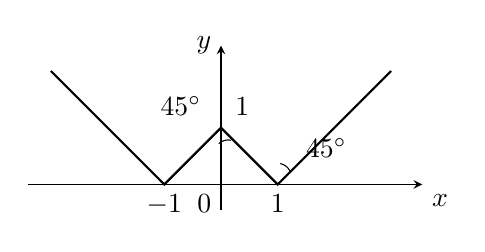
\begin{tikzpicture}[scale=0.72,>=stealth]
  \draw[->] (-3.4,0)--(3.55,0) node[below right] {$x$};
  \draw[->] (0,-0.45)--(0,2.45) node[left] {$y$};
  \draw[thick] (-3.0,2)--(-1,0)--(0,1)--(1,0)--(3.0,2);
  \draw (0.18,0.78) arc (78:132:0.25);
  \draw (1.22,0.23) arc (25:78:0.25);
  \node[above right] at (0.08,1.05) {$1$};
  \node[below left] at (0,0) {$0$};
  \node[below] at (-1,0) {$-1$};
  \node[below] at (1,0) {$1$};
  \node[above left] at (-0.18,1.05) {$45^\circ$};
  \node[above right] at (1.33,0.30) {$45^\circ$};
\end{tikzpicture}
\end{center}
\nopagebreak[4]
那么 $f(x)=$\mbox{（　　）}

（A）$\sqrt{x^2-2x+1}$　　（B）$\sqrt{x^2-2|x|+1}$

（C）$|x^2-1|$　　（D）$x^2-2|x|+1$

\Needspace{5\baselineskip}
（25） 设点 $A(-2,\sqrt3)$，$F$ 为椭圆

\nopagebreak[4]
\[
\frac{x^2}{16}+\frac{y^2}{12}=1
\]

的右焦点，点 $M$ 在该椭圆上移动，当 $|AM|+2|MF|$ 取最小值时，点 $M$ 的坐标是\mbox{（　　）}

（A）$(0,2\sqrt3)$　　（B）$(0,-2\sqrt3)$

（C）$(2\sqrt3,\sqrt3)$　　（D）$(-2\sqrt3,\sqrt3)$

\end{question}
\begin{question}
\gkti{2}

第二卷第一题（本题满分 15 分）共有 5 个小题，每小题满分 3 分。每个小题都有用横线表示的空位，请把你认为合适的内容写在横线上的空位里。

（1） 已知点 $A(1,0)$ 和 $B(2,1)$，那么线段 $AB$ 的垂直平分线方程是　　　　。

\Needspace{5\baselineskip}
（2）　

\nopagebreak[4]
\[
\cos10^\circ\cos55^\circ+\cos80^\circ\cos35^\circ
\]

的值等于　　　　。

（3） 函数 $y=|\sin x|$ 的最小正周期是　　　　。

\Needspace{5\baselineskip}
（4） 设复数

\nopagebreak[4]
\[
z=2\left(\cos\frac\pi6+i\sin\frac\pi6\right),
\]

那么，$z$ 的共轭复数 $\overline z$ 的代数形式是　　　　。

\Needspace{5\baselineskip}
（5）　

\nopagebreak[4]
\[
\lim_{n\to\infty}
\frac{1-2+3-4+\cdots+(2n-1)-2n}{n-1}
\]

的值是　　　　。

\end{question}
\begin{question}
\gkti{3}

\Needspace{5\baselineskip}
第二卷第二题（本题满分 13 分）。设复数

\nopagebreak[4]
\[
z=-\sqrt6+\sqrt2i,
\]

\Needspace{5\baselineskip}
记

\nopagebreak[4]
\[
u=\left(\frac4z\right)^3.
\]

（1） 求 $|u|$ 和 $\arg u$ 的值。

\Needspace{5\baselineskip}
（2） 求实数 $x$ 和 $y$，使

\nopagebreak[4]
\[
\frac{x}{z}+\frac{y}{u}=z+2u.
\]

\Needspace{0.4\textheight}
\end{question}
\begin{question}
\gkti{4}

第二卷第三题（本题满分 14 分）。如图，在四棱锥 $P-ABCD$ 中，$PA\perp$ 底面 $ABCD$，$PD\perp DC$，$DC\parallel$ 侧面 $PAB$。
\nopagebreak[4]
\begin{center}% 1988 年广东卷文史类第二卷第二题：四棱锥 P-ABCD
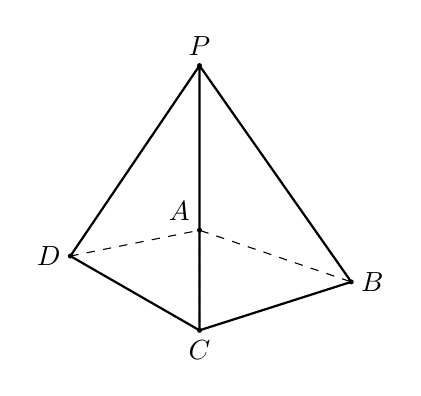
\begin{tikzpicture}[scale=0.82,>=stealth]
  \coordinate (P) at (2.0,4.1);
  \coordinate (D) at (0,1.15);
  \coordinate (C) at (2.0,0);
  \coordinate (B) at (4.35,0.75);
  \coordinate (A) at (2.0,1.55);
  \draw[thick] (P)--(D) (P)--(C) (P)--(B);
  \draw[dashed] (P)--(A);
  \draw[thick] (D)--(C)--(B);
  \draw[dashed] (D)--(A)--(B) (A)--(C);
  \fill (P) circle (1.1pt) node[above] {$P$};
  \fill (A) circle (1.1pt) node[above left] {$A$};
  \fill (B) circle (1.1pt) node[right] {$B$};
  \fill (C) circle (1.1pt) node[below] {$C$};
  \fill (D) circle (1.1pt) node[left] {$D$};
\end{tikzpicture}
\end{center}
\nopagebreak[4]
（1） 求证：$DA\perp AB$。

（2） 又设 $PB=PC$，且 $DC=PA=3\,\mathrm{cm}$，$DA=4\,\mathrm{cm}$，求这个四棱锥的体积。

\end{question}
\begin{question}
\gkti{5}

\Needspace{5\baselineskip}
第二卷第四题（本题满分 14 分）。设数列 $\{a_n\}$ 的前 $n$ 项和

\nopagebreak[4]
\[
S_n=\frac\pi3n^2+c,
\]

式中 $c$ 是常数，$n=1,2,\ldots$。

（1） 如果 $c\ne0$，求证：$\{a_n\}$ 不是等差数列。

\Needspace{5\baselineskip}
（2） 如果 $c=0$，求证：对任意大于 1 的自然数 $n$，和数

\nopagebreak[4]
\[
\cos^2(a_{n-1})+\cos^2(a_n)+\cos^2(a_{n+1})
\]

是一个与 $n$ 无关的常数，并求出这个常数值。

\end{question}
\begin{question}
\gkti{6}

\Needspace{5\baselineskip}
第二卷第五题（本题满分 14 分）。设 $k$ 和 $r$ 是实数，且 $r>0$，使得：直线 $y=kx+1$ 既与圆

\nopagebreak[4]
\[
x^2+y^2=r^2
\]

\Needspace{5\baselineskip}
相切，又与双曲线

\nopagebreak[4]
\[
x^2-y^2=r^2
\]

有两个交点。

（1） 求证：$\dfrac1{r^2}-k^2=1$，且 $|k|\ne1$。

（2） 试问：直线 $y=kx+1$ 能否经过双曲线 $x^2-y^2=r^2$ 的焦点？为什么？

\end{question}